\subsubsection{bringit::client::view::list::create::CreateListView}

\label{bringit::client::view::list::create::CreateListView}
\begin{figure}[H]
	\centering
	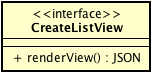
\includegraphics[scale=0.5]{Sezioni/SottosezioniST/img/app/CreateListView.png}
	\caption{bringit::client::view::list::create::CreateListView}
\end{figure}

\begin{itemize}
\item \textbf{Descrizione}: La view relativa alla parte grafica di creazione di una lista.
\item \textbf{Utilizzo}: L'interfaccia viene utilizzata per disaccoppiare presenter e implementazione della classe e per visualizzare i dati che gli vengono passati dal presenter.
\item \textbf{Attributi}: 
\item \textbf{Metodi}:
	\begin{itemize}
	\item \textit{public renderView():JSONObject}\\
	Il metodo ritorna un file JSON necessario per la visualizzazione del bottone di creazione della lista bringit.
	\end{itemize}
\end{itemize} 

\subsubsection{bringit::client::view::list::create::view::CreateListViewImpl}

\label{bringit::client::view::list::create::view::CreateListViewImpl}
\begin{figure}[H]
	\centering
	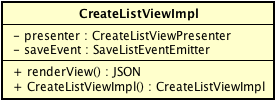
\includegraphics[scale=0.5]{Sezioni/SottosezioniST/img/app/CreateListViewImpl.png}
	\caption{bringit::client::view::list::create::view::CreateListViewImpl}
\end{figure}

\begin{itemize}
\item \textbf{Descrizione}: Questa classe rappresenta il bottone utilizzato per la creazione della lista bringit.
\item \textbf{Utilizzo}: Implementando i metodi di CreateListViewImpl questa classe viene utilizzata al momento dell'inserimento delle informazioni relative ad un item della lista bringit.
\item \textbf{Attributi}: 
\begin{itemize}
	\item \textit{private presenter:CreateListViewPresenter}\\
	Il presenter relativo alla creazione di una lista.
	\item \textit{private saveEvent:SaveEventEmitter}\\
	Il riferimento all'oggetto responsabile dell'emissione degli eventi di salvataggio su database.
\end{itemize}
\item \textbf{Metodi}:
	\begin{itemize}
	\item \textit{public CreateListViewImpl():CreateListViewImpl}\\
	Il costruttore di CreateListViewImpl.
	\item \textit{public renderView():JSONObject}\\
	Il metodo ritorna un file JSON necessario per la visualizzazione del bottone di creazione della lista bringit.
	\end{itemize}
\end{itemize} 

\subsubsection{bringit::client::view::list::create::presenter::CreateListViewPresenter}

\label{bringit::client::view::list::create::presenter::CreateListViewPresenter}
\begin{figure}[H]
	\centering
	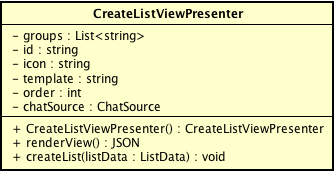
\includegraphics[scale=0.5]{Sezioni/SottosezioniST/img/app/CreateListViewPresenter.png}
	\caption{bringit::client::view::list::create::presenter::CreateListViewPresenter}
\end{figure}

\begin{itemize}
\item \textbf{Descrizione}: Questa classe rappresenta il presenter per la classe di creazione della lista bringit.
\item \textbf{Utilizzo}: Il presenter fa da tramite tra l'implementazione e la view, formattando i dati che verranno visualizzati nella view e manipolando gli input dell'utente per eseguire le operazioni logiche predisposte.
\item \textbf{Attributi}: 
	\begin{itemize}
	\item \textit{private groups:string[]}\\
	Array che specifica la posizione del bottone di creazione della lista (ovvero canali, gruppi e messaggi diretti).
	\item \textit{private id:string}\\
	Identificativo del bottone di creazione della lista.
	\item \textit{private icon:string}\\
	Il nome dell'icona utilizzata per visualizzare il bottone di creazione della lista.
	\item \textit{private template:string}\\
	Il nome del template HTML che appare alla pressione del bottone.
	\item \textit{private order:number}\\
	Il numero che rappresenta la posizione del bottone sulla colonna laterale di Rocket.Chat.
	\item \textit{private chatSource:ChatSource}\\
	Il riferimento alla classe necessaria per interfacciarsi a Rocket.Chat.
	\end{itemize}
\item \textbf{Metodi}:
	\begin{itemize}
	\item \textit{public CreateListViewPresenter():CreateListViewPresenter}\\
	Il costruttore di CreateListViewPresenter.
	\item \textit{public renderView():JSONObject}\\
	Il metodo ritorna un file JSON necessario per la visualizzazione del bottone di creazione della lista bringit.
	\item \textit{public createList(listData:ListData):void}\\
	Questo metodo manda un messaggio con una lista trasformata in JSON.
				\\ \textbf{Parametri}: \begin{itemize}
			\item \textit{listData:ListData}\\
			La lista che viene trasformata in JSON e mandata alla chat.
					\end{itemize} 
	\end{itemize}
\end{itemize} 
